\chapter{背景}

本章では、Multilayer~perceptron及びその応用例のGenerative~Adversarial~Networksの説明を行った後、Generative~Adversarial~Networksを画像の変換に応用したPix2pixを紹介する。

\section{Multilayer~perceptron}

Multilayer~perceptron~(MLP)~は複数のアフィン変換と非線形関数からなる関数により定義され、式\ref{eq:MLP}で定式化される。

\begin{align}
    \label{eq:MLP}
    F_{MLP}(\boldsymbol{x})&=f_{n}(W_{n}(f_{n-1}(W_{n-1}\cdots(f_{1}(W_{1}\boldsymbol{x}+\boldsymbol{b_{1}}))\cdots+\boldsymbol{b_{n-1}}))+\boldsymbol{b_{n}})
\end{align}

ここで、$\boldsymbol{x}$は実数ベクトル,$n$は1以上の整数,$f_{i}$は$i$番目の非線形関数,$W_{i}$は$i$番目の行列,$b_{i}$は$i$番目の定数ベクトルである。また、$n$を層数と呼ぶ。


%Adam,SGDもちゃんと学ぶ

MLP~($F_{MLP}$)~を用いると、あるデータ集合$D=\{(\boldsymbol{x_j},\boldsymbol{t_j}); 1 \leqq j \leqq N\}$について、それぞれの$j$で$\boldsymbol{t_{j}}$の予測値として$\boldsymbol{y_j}=F_{MLP}(\boldsymbol{x_j})$を出力することができる。しかし、$\boldsymbol{t_j}$に近い$\boldsymbol{y_j}$を出力するためにはそれぞれの$i$で$W_i$を適切に決める必要がある。損失関数$L(\boldsymbol{y_j},\boldsymbol{t_j})$を定義し、$W _i \leftarrow W_i - \eta \frac{d L}{dW_i}$として更新すると、$\boldsymbol{y_j}$を$\boldsymbol{t_j}$に近づける方向に$W_i$を更新することができる~(勾配降下法)~。ここで、$\eta$は任意の正の実数であり、学習率と呼ばれている。なお、この学習率を適切に設定するためにStochastic Gradient Descent~\cite{SGD}やAdam~\cite{Adam}などのアルゴリズムが用いられる。また、損失関数としては、平均二乗誤差$L_{MSE}=\frac{1}{n}\sum _{j=1} ^{n} {(\boldsymbol{y_j} - \boldsymbol{t_j})^2}$や平均絶対誤差$L_{MAE}=\frac{1}{n}\sum _{j=1} ^{n} {|\boldsymbol{y_j} - \boldsymbol{t_j}|}$などが用いられる。

一般には、ニューラルネットワークはMLPより広い概念であるが、本論文ではこれ以降MLPのことをニューラルネットワークと呼ぶ。

\section{Generative~Adversarial~Networks}

\begin{figure}[t]
\begin{center}
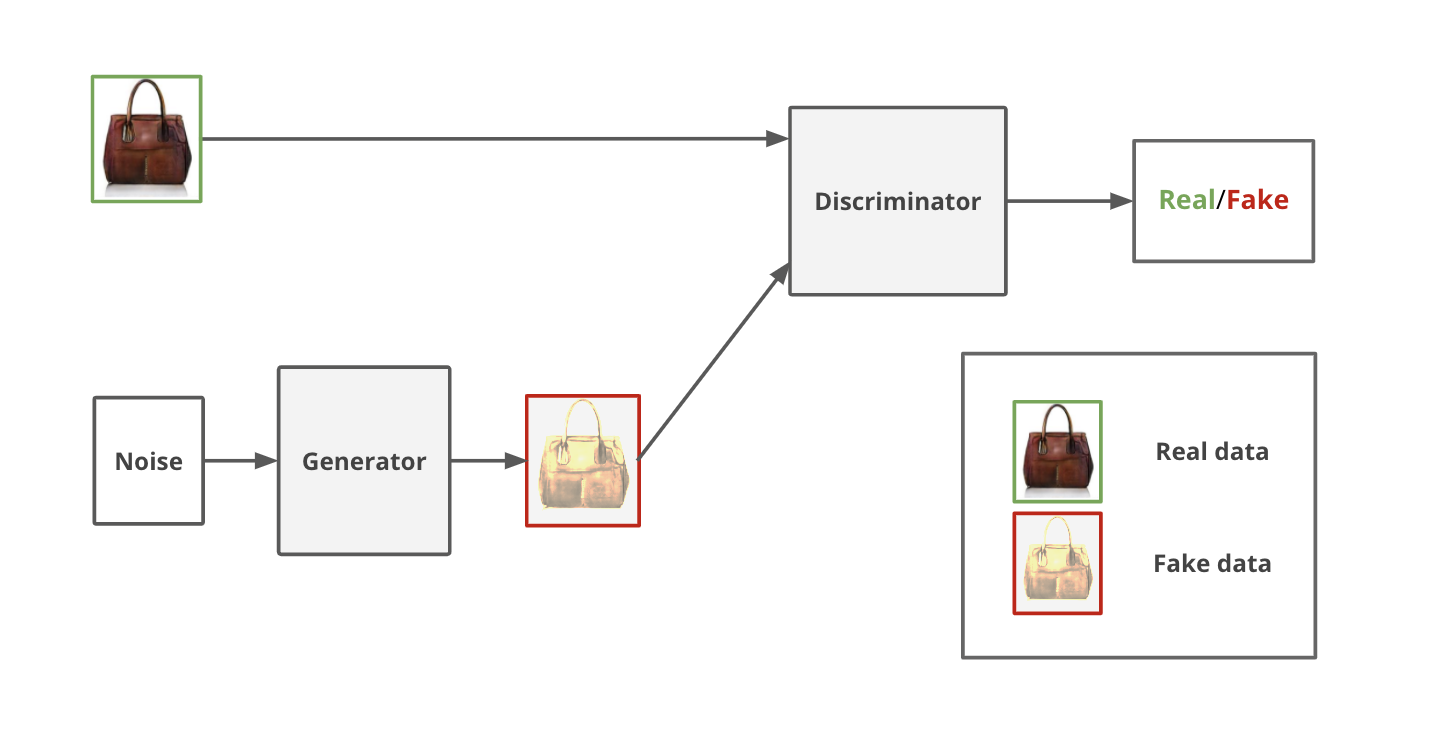
\includegraphics[width=\hsize]{figure/GAN_net.png}
\caption{GANのネットワーク}
\label{fig:GAN_net}
\end{center}
\end{figure}


Generative~Adversarial~Networks~(GAN)~\cite{GAN}はニューラルネットワークの応用例であり、学習データの特徴を学習して擬似的なデータを生成することを目指す手法である。この手法は自然な手書きの文字を出力する際などに用いられる。

GANは二つのニューラルネットワークで構成され、それぞれ識別モデルと生成モデルと呼ばれる。この二つのモデルはランダムに初期化された後に競合的に学習を進める。まず、識別モデルはデータが生成モデルの出力と学習データのどちらであるかを識別できるように学習を進める。そして、生成モデルは識別モデルが学習データであると誤って識別するよう学習データに近いデータを出力する。この二つの学習を交互に繰り返すことで、漸進的に生成モデルが学習データにより近いデータを生成できるようになると期待される。

生成モデルの目的関数は式\ref{eq:GAN_G},識別モデルの目的関数は式\ref{eq:GAN_D}として定式化される。

\begin{align}
    \label{eq:GAN_G}
    \argmin _{\theta_G}& \mathbb{E}_{\boldsymbol{z}}[\log (1-D(G(\boldsymbol{z};\theta_G);\theta_D))]\\
    \label{eq:GAN_D}
    \argmax _{\theta_D}& \mathbb{E}_{\boldsymbol{x}}[\log D(\boldsymbol{x};\theta_D)]+\mathbb{E}_{\boldsymbol{z}}[\log (1-D(G(\boldsymbol{z};\theta_G);\theta_D))]
\end{align}


ここで、$\boldsymbol{x}$は学習データ,$\boldsymbol{z}$は生成モデルへの入力のノイズ,$G(\boldsymbol{z};\theta_G)$はノイズ$\boldsymbol{z}$を入力とする生成モデル,$D(\cdot;\theta_D)$は識別モデル,$\theta_G$は生成モデル$G$のパラメータ,$\theta_D$は識別モデル$D$のパラメータである。ここで、ノイズ$\boldsymbol{z}$は生成モデルの出力データの揺らぎを表現する元となる潜在変数である。

\section{Pix2pix}

\begin{figure}[t]
\begin{center}
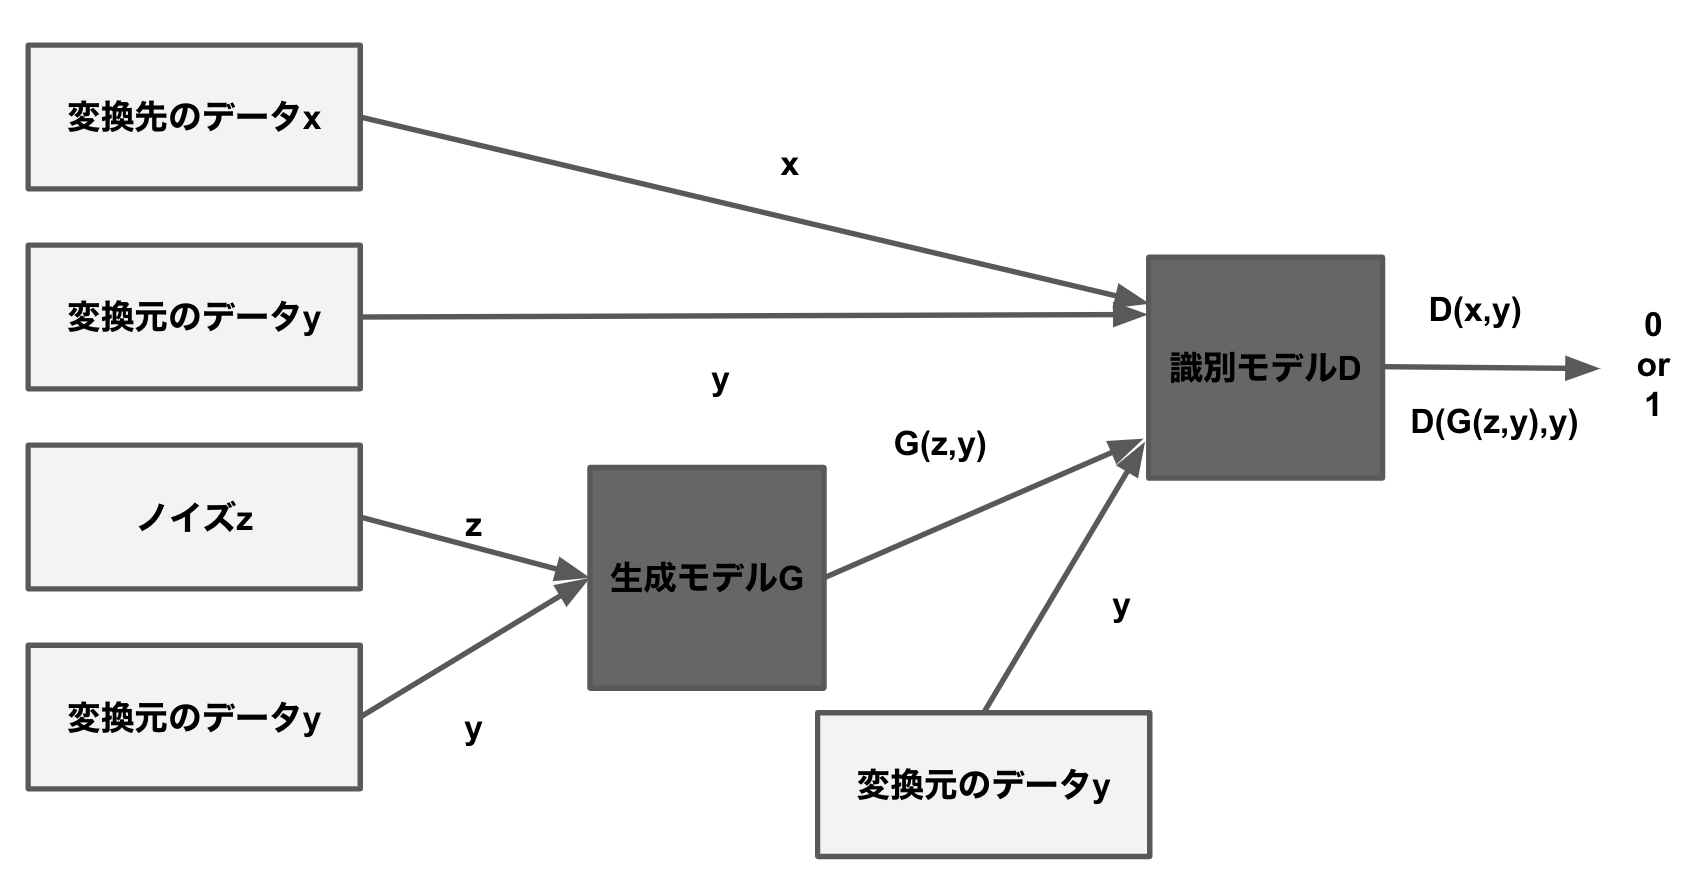
\includegraphics[width=\hsize]{figure/pix2pix_net.png}
\caption{pix2pixのネットワーク}
\label{fig:pix2pix_net}
\end{center}
\end{figure}

\begin{figure}[t]
\begin{center}
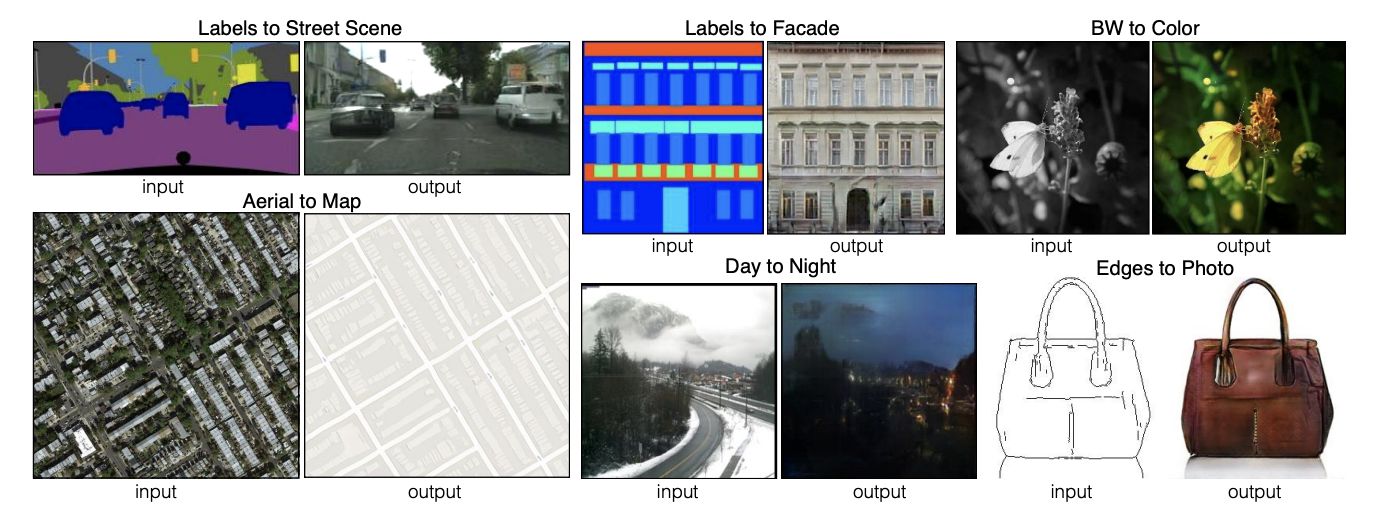
\includegraphics[width=\hsize]{figure/pix2pix_img.png}
\caption{pix2pixのスタイル変換の例}
\label{fig:pix2pix_img}
\end{center}
\end{figure}

Pix2pix~\cite{pix2pix}はある条件下で画像間の変換を行うGANである。特定の条件の元で用いるGANとしてはConditional~GAN~(CGAN)~\cite{CGAN}が初めて考案されたが、Pix2pixは与えられた条件の構造を維持したまま画像を変換するという点でCGANとは異なる。具体的には、Pix2pixは図\ref{fig:pix2pix_img}のようにピクセルの対応関係を変えずにスタイル変換を行うことができる。Pix2pixはGANに変換先の学習データを条件として与えることでスタイル変換を行い、生成モデルの目的関数は式\ref{eq:pix2pix_G},識別モデルの目的関数は式\ref{eq:pix2pix_D}でとして定式化される。

\begin{align}
    \label{eq:pix2pix_G}
    \argmin _{\theta_G}& \mathbb{E}_{\boldsymbol{y}, \boldsymbol{z}}[\log (1-D(\boldsymbol{y}, G(\boldsymbol{y}, \boldsymbol{z}; \theta_G); \theta_D))]+\mathbb{E}_{\boldsymbol{x}, \boldsymbol{y}, \boldsymbol{z}}[\|\boldsymbol{x}-G(\boldsymbol{y}, \boldsymbol{z}; \theta_G)\|_{1}]\\
    \label{eq:pix2pix_D}
    \argmax _{\theta_D}& \mathbb{E}_{\boldsymbol{x}, \boldsymbol{y}}[\log D(\boldsymbol{x}, \boldsymbol{y}; \theta_D)]+\mathbb{E}_{\boldsymbol{y}, \boldsymbol{z}}[\log (1-D(\boldsymbol{y}, G(\boldsymbol{y}, \boldsymbol{z}; \theta_G); \theta_D))]
\end{align}


ここで、$\boldsymbol{x}$は変換先の学習データ,$\boldsymbol{y}$は変換元の学習データ,$\boldsymbol{z}$は生成モデルへの入力のノイズ,$G(\boldsymbol{y},\boldsymbol{z};\theta_G)$は$\boldsymbol{y}$を条件としノイズ$\boldsymbol{z}$を入力とする生成モデル,$D(\boldsymbol{y},\cdot;\theta_D)$は$\boldsymbol{y}$を条件とする識別モデル,$\theta_G$は生成モデル$G$のパラメータ,$\theta_D$は識別モデル$D$のパラメータである。

\subsection{生成モデルの構造}

\begin{figure}[t]
\begin{center}
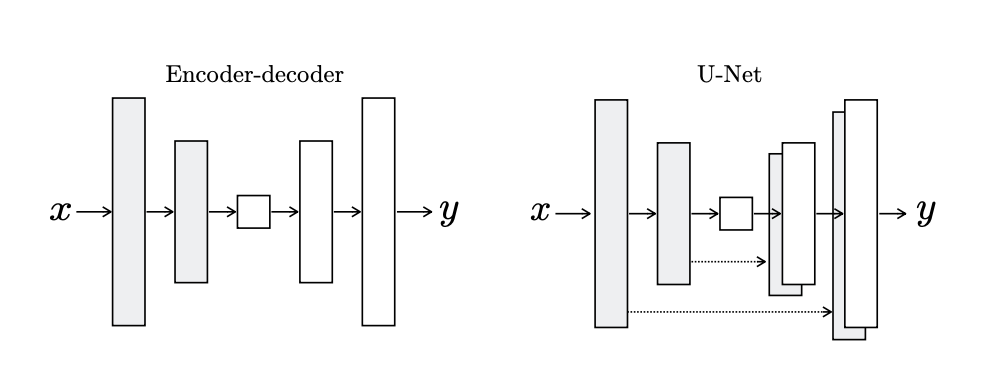
\includegraphics[width=\hsize]{figure/u-net.png}
\caption{Encoder-decoderのネットワークとU-netのネットワーク。図は文献~\cite{u-net}の図の〇〇から引用。}
\label{fig:u-net}
\end{center}
\end{figure}

%Encoder-Decoderのネットワーク例をciteする

変換を行うための生成モデルにはEncoder-decoderのネットワークが用いられる。Pix2pixの生成モデルでは、画像データの基礎的な構造を保持するために、図\ref{fig:u-net}のようにU-net\cite{u-net}というスキップコネクションを持ったネットワークが用いられる。

\subsection{識別モデルの構造}

%直感的な図を貼る

Pix2pixの識別モデルでは、PatchGANという手法が用いられる。PatchGANは画像全体の誤差を求めるのではなくパッチと呼ばれる小領域ごとで誤差を求めて平均を取っている。これにより、局所的な部分の識別の精度が高まることが期待される。

